In this section, the problem of multistream classification with domain adaptation is finalized, and the challenges of conducting an adaptive classification performance over concept drifting data streams is presented.

\begin{figure}[t]
\centering
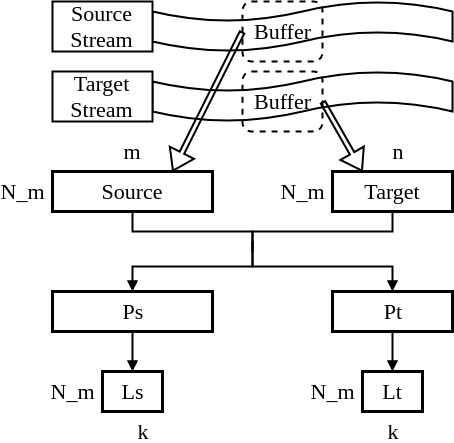
\includegraphics[width=0.7\columnwidth]{Figures/domain_adaptation.png}
\caption{Feature Projection}
\label{fig:domainadaptation}
\end{figure}


\subsection{Notations and Problem Statement}
\label{subsec: problemstatement}

In Table~\ref{tab:notations}, frequently used symbols in this paper are listed. There are two 
continuous stream of data instances generated from source domain $D_{s}$ and target domain $D_{t}$.
A data instance is denoted as $(x, y)$, where $x$ is a vector ($m$-dimensional in 
source stream and $n$-dimensional in target stream), and $y$ is the 
corresponding class label. In the source stream, both $x_{s}$ and $y_{s}$  are available, while in the target domain only $x_{t}$ is available. Therefore, a multistream classification with domain adaptation problem can be described as follows:

Suppose $X_{s}$ is a set of $m$-dimensional vectors and $Y_{s}$ is the corresponding labels in a source stream from a certain domain $D_{s}$, 
whereas $X_{t}$ is a set of $n$-dimensional vectors in target stream from another 
domain $D_{t}$. In our problem setting, $m\neq n$. The objective is to construct a classifier $M$ that
predicts class labels of $x_{t} \in X_{t}$ using $X_{s}$, and $Y_{s}$.

\begin{table}[t]
\centering
\caption{Notations}
\label{tab:notations}
\begin{tabular}{|l|l|}
\hline
Symbol & Meaning \\ \hline
 $D_{s}$ & Domain of source stream \\ \hline
 $D_{t}$ & Domain of target stream \\ \hline
 $S$ & Source stream data\\ \hline
 $T$ & Target stream data \\ \hline
 $X_{s}$, $X_{t}$ & Feature space of source stream with dimension $m$, \\
  & and that of target stream with dimension $n$\\ \hline
 $Y_{s}$, $Y_{t}$ & Label space of source and target stream \\ \hline
 $x_{s}$, $x_{t}$ & Data instance of source and target stream \\ \hline
 $y_{s}$, $y_{t}$ & True/predicted label of a data instance in source stream \\ \hline
 $W_{s}$, $W_{t}$ & Projection function to the source and target space \\ \hline
 $L_{s}$, $L_{t}$ & Projected data from source and target domain to latent space \\ \hline
 $P_{s}$, $P_{t}$ & Probability distribution function of source and target data \\ \hline 
 $N_{m}$ & Size of sliding window \\ \hline
\end{tabular}
\end{table}

\subsection{Challenges}
In the problem setting of multistream classification with domain adaptation, there are two major challenges at the same time.
The first challenge is the adaptation of both source and target domain, and it can be represented as $D_{s} \neq D_{t}$. As shown in Figure~\ref{fig:domainadaptation}, two streams may have different number of instances. However, without loss of generality, buffers (windows) from these streams representing contiguous data points will have the same number of instances $N_m$. Furthermore, each data point in source stream may have a different number of features compared to those in the target stream.

Therefore, source data cannot be directly used as training data to learn the target task, 
and discovering a latent feature space with $k$ dimensions is the key to handling the feature heterogeneity issue.
The second challenge is the asynchronous concept drift in both source and target streams. 
This phenomenon means that the data pattern evolves, or more formally, the conditional probability distribution changes over time in both streams. 
Here, the problem can be described as $P_{s}^{t}(y \mid \mathbf{x}) \neq P_{t}^{t}(y \mid \mathbf{x})$ at time $t$. Furthermore, we assume that source and target data streams have asynchronous concept drifts,
which means that the drifts in both streams occur independently. 

% \textcolor{red}{add detailed demonstration of the flow chart here}
